In order to address the problem raised by Herley, 
we shall define how to distinguish between a secure and an insecure system.
While most of the literature (and this paper so far) have
correlated the problem of in-security to the maliciousness of
agents interacting with the system, we show that security
doesn't seem to have a malicious nature but, rather, insecurity 
raises from the lack of well-defined security requirements for the
design process of a system. We argue that the high number
of security vulnerability reported today are simply the realization
of potential system configurations, which deviate from the unintended 
behavior just because the intended behavior of the system is not precisely 
defined in the specification of the design process.

Given that the application of our theory is \emph{systems engineering} and that
the two foundational processes (exploitation and hacking) are based on the
concept of a system, we shall begin by defining what a system is, in its
abstract form.

\subsection{Abstract Systems}\label{sec:system}
The ISO/IEC/IEEE 15288:2015 (System Life Cycle Processes) 
provides a definition of system as ``A combination of interacting elements organized to
achieve one or more stated purposes.''\autocite{ISO201515288}.
Therefore, a system can be considered as a single agent where it's interacting
elements are the constituents of the agent itself. For the sake of simplicity
we first define a system as an agent and then extend the definition
to a ``combination of interacting'' agents.

We use the same process of \autocite{Santaca2016abf} but over slightly different
terms. The differences and commonalities with \autocite{Santaca2016abf} 
are described in Appendix~\ref{app:abf}. There is no 
agreement between the research communities (e.g. Multi-Agent-System, Epistemic Logic)
on which are the constituent of an agent as a system. However,
the same ideas revolved around for thousands of years. Some examples
follows.
\begin{itemize}
	\item In \autocite{Georgeoff1995bdi}, the BDI (Belief, Desire, Intent)
		paradigm is explained; where an agent can be defined over those
		three constituents.
	\item In \autocite{Hintikka1962knwoledge}, Hintikka describes the
		difference between Knowledge and Belief (as epistemological
		concepts), and the whole Doxastic logic defines in details how
		Beliefs can be formalized.
	\item In \autocite{Hintikka1993Information}, Hintikka describes the concept
		of Information and the difference with Knowledge and Belief.
	\item In \autocite{Empiricus1990Pyrrhonism}, the author states: ``The
		logical criterion also may be used in three senses -- of the
		agent, or the instrument, or the ``according to what''; the
		agent, for instance, may be a man, the instrument either sense
		perception or intelligence, and the ``according to what'' the
		application of the impression ``according to'' which the man
		proceeds to judge by means of one of the aforesaid
		instruments.'' 
	\item In \autocite{Santaca2016abf}, the authors defines an agent as a
		tuple of Assertions, Beliefs, and Facts.
\end{itemize}

\begin{figure}[t]
	\centering
	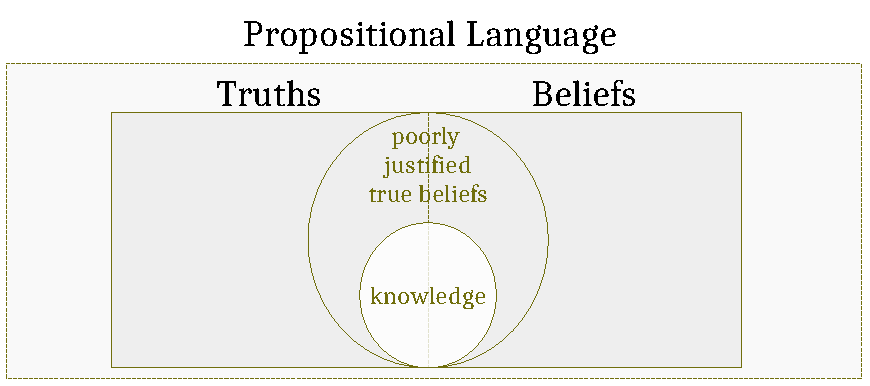
\includegraphics[width=.8\textwidth]{knowledge-belief.pdf}
	\caption{Informal representation of Knowledge and Belief}
	\label{fig:knowledge-belief}
\end{figure}

\subsubsection{Region: Threat and Asset}\label{sec:threatasset}
The difference between Knowledge and Belief is depicted in
Figure~\ref{fig:knowledge-belief} (see \autocite{wiki-knowledgebelief}).  However,
according to\autocite{Gettier2012knowledge},
Knowledge\footnote{``\emph{Theaetetus}: [\ldots] He said that knowledge was
true opinion accompanied by reason, but that unreasoning true opinion was
outside of the sphere of knowledge; and matters of which there is not a
rational explanation are unknowable -- yes, that is what he called them -- and
those of which there is are knowable. [\ldots] \emph{Socrates}: [\ldots] the
primary elements of which we and all else are composed admit of no rational
explanation; for each alone by itself can only be named, and no qualification
can be added, neither that it is nor that it is not, for that would at once be
adding to it existence or non-existence, whereas we must add nothing to it, if
we are to speak of that itself alone.  [\ldots]'' Plato -- Theaetetus 201
\autocite{Plato1914Plato}} as an epistemological concept is difficult (and
sometimes believed impossible\autocite{citation}) to formally define. In this
work, we are not interested in 
how knowledge can be precisely formalized from an epistemic standpoint. 
We assume that a semantic of a correct definition of epistemic knowledge exists,
for example the one given in\autocite{Hintikka1962knwoledge} by Hintikka, and we then define 
knowledge in terms of the Kripke structure defined in Definition~\ref{def:causality}.

\begin{definition}{\bf Knowledge --}\label{def:knowledge}
Given an abstract collection of Agents $Ag$, and the modal operator
	$\knows{a}{}$ (where $a\in Ag$), Knowledge is defined as a collection
	of predicates known by an agent $\knowledge{a}=\bigcup_\Phi \knows{a}{\varphi}$ 
	(where $\Phi$ is the collection of all the propositions known by $a$).
	Given a proposition $P$, we extend the semantics of the Causality structure with:
	\begin{enumerate}[noitemsep]
		\item[$(\interpretation6)$] $\world\models\knows{a}{P}$ iff
			$\world'\models P$ for all $\world'$ such that
			$\world\modalrelation\world'$.
	\end{enumerate}
\end{definition}

\begin{definition}{\bf Belief --}\label{def:belief}
	\fix{mr}{we should help the reader in understanding the upgrades of the logic. We used propositional with modal operators with a K Kripke semantics and we are now introducing Belief as in Doxastic logic? and we have epistemological operators as knowledge}
	Given an abstract collection of Agents $Ag$, and the modal operator
	$\believe{a}{}$ (where $a\in Ag$), Belief is defined as a collection
	of predicates believed by an agent $\belief{a}=\bigcup_\Phi \believe{a}{\varphi}$
	(where $\Phi$ is the collection of all the propositions believed by $a$).
	Given a proposition $P$, we extend the semantics of the Causality structure with:
	\begin{enumerate}[noitemsep]
		\item[$(\interpretation7)$] $\world\models\believe{a}{P}$ iff
			$\world\models\neg\knows{a}{\neg P}$ (i.e. the agent $a$ considers $P$ possible) 
			and $\world'\models P$ for all
			$\world'$ such that $\world\modalrelation\world'$.
	\end{enumerate}
\end{definition}

\begin{definition}{\bf Mankind/Nature --}\label{def:mankind-nature}
Mankind/Nature is represented as an agent.  
	%countable logical signature $\Sigma_M$/$\Sigma_N$ over an
	%abstract algebraic structure.  We also consider a countable signature
	%of variables, disjoint from $\Sigma_M$/$\Sigma_N$, and write
	%$\Sigma_{M_n}$/$\Sigma_{N_n}$ for the symbols of $\Sigma_M$/$\Sigma_N$
	%with arity $n$. Thus, $\Sigma_0$ is a collection of constants, which we
	%assume to have disjoint sub-collections that we refer to as
	%\emph{sub-agents} of Mankind or Nature (i.e. humans, plants, \&c).
	%The variables are untyped and can be instantiated with arbitrary types,
	%yielding an untyped model.
\end{definition}

\subsubsection{Mereotopological Representation of Safety and Security}\label{sec:formalGlossary}
The objectives of this section are:
\begin{enumerate}[noitemsep]
	\item formalize the abstract algebraic structure (as a mereotopology)
		on top of which we have formalized the terms in
		Figure~\ref{fig:safety-security} so far, i.e. Mankind, Nature,
		Truths, Beliefs, and Knowledge.
	\item correlate mereological structure to Causality and then Kripke
		structure by defining the relation $R$ over the Kripke
		structure as the mereotopological basic relation connects with,
		i.e. reflexive and symmetric
	\item we map signature to mereotopological Regions to express the
		logical formulation of terms (e.g. Mankind, Nature, Truths,
		Beliefs, Knowledge, Vulnerabilities) over the mereotopological
		structure
	\item we formalize the relations between terms using the RCC(5)
\end{enumerate}

\fix{mr}{change propositions in propositional language\url{http://logic.stanford.edu/intrologic/lectures/lecture_02.pdf}}

Given that the concepts of Truths, Beliefs, and Knowledge are positioned over
an underlying structure of Propositions, the first concept to formalize is that
of Propositions. We do not restrict Propositions to a specific structure but,
as for Mankind and Nature, we refer to them as a collection.  We express the
generality of a collection as a (propositional) signature over an abstract
algebraic structure. In our formalization, we use mereotopology as algebraic
structure (due to its generality, as discussed in Section~\ref{sec:problem})
and the RCC to formalize concepts over a mereotopology. 

We can now define the possible mereotopological relations between Belief and
Knowledge (informally depicted in Figure~\ref{fig:knowledge-belief}) and then
define the peculiarity of the believed difference between Mankind and Nature 
(i.e. maliciousness as intent). 
We first start from the formalization of Figure~\ref{fig:knowledge-belief}, as
follows.  

\begin{definition}{\bf Information}\label{def:information}
\end{definition}
\begin{definition}{\bf Desire}\label{def:desire}
\end{definition}
\begin{definition}{\bf Intent}\label{def:intent}
\end{definition}
